The experimental layout used throught the measurements is presented figure \ref{fig:exp_lay}. 
The layout is designed to allow interchanging light sources incident on the SPAD. 
Optical elements can also be introduced between the source and the SPAD for attenuation, modulation and alignment purposes.\\   

\begin{figure}[htpb]
    \centering
    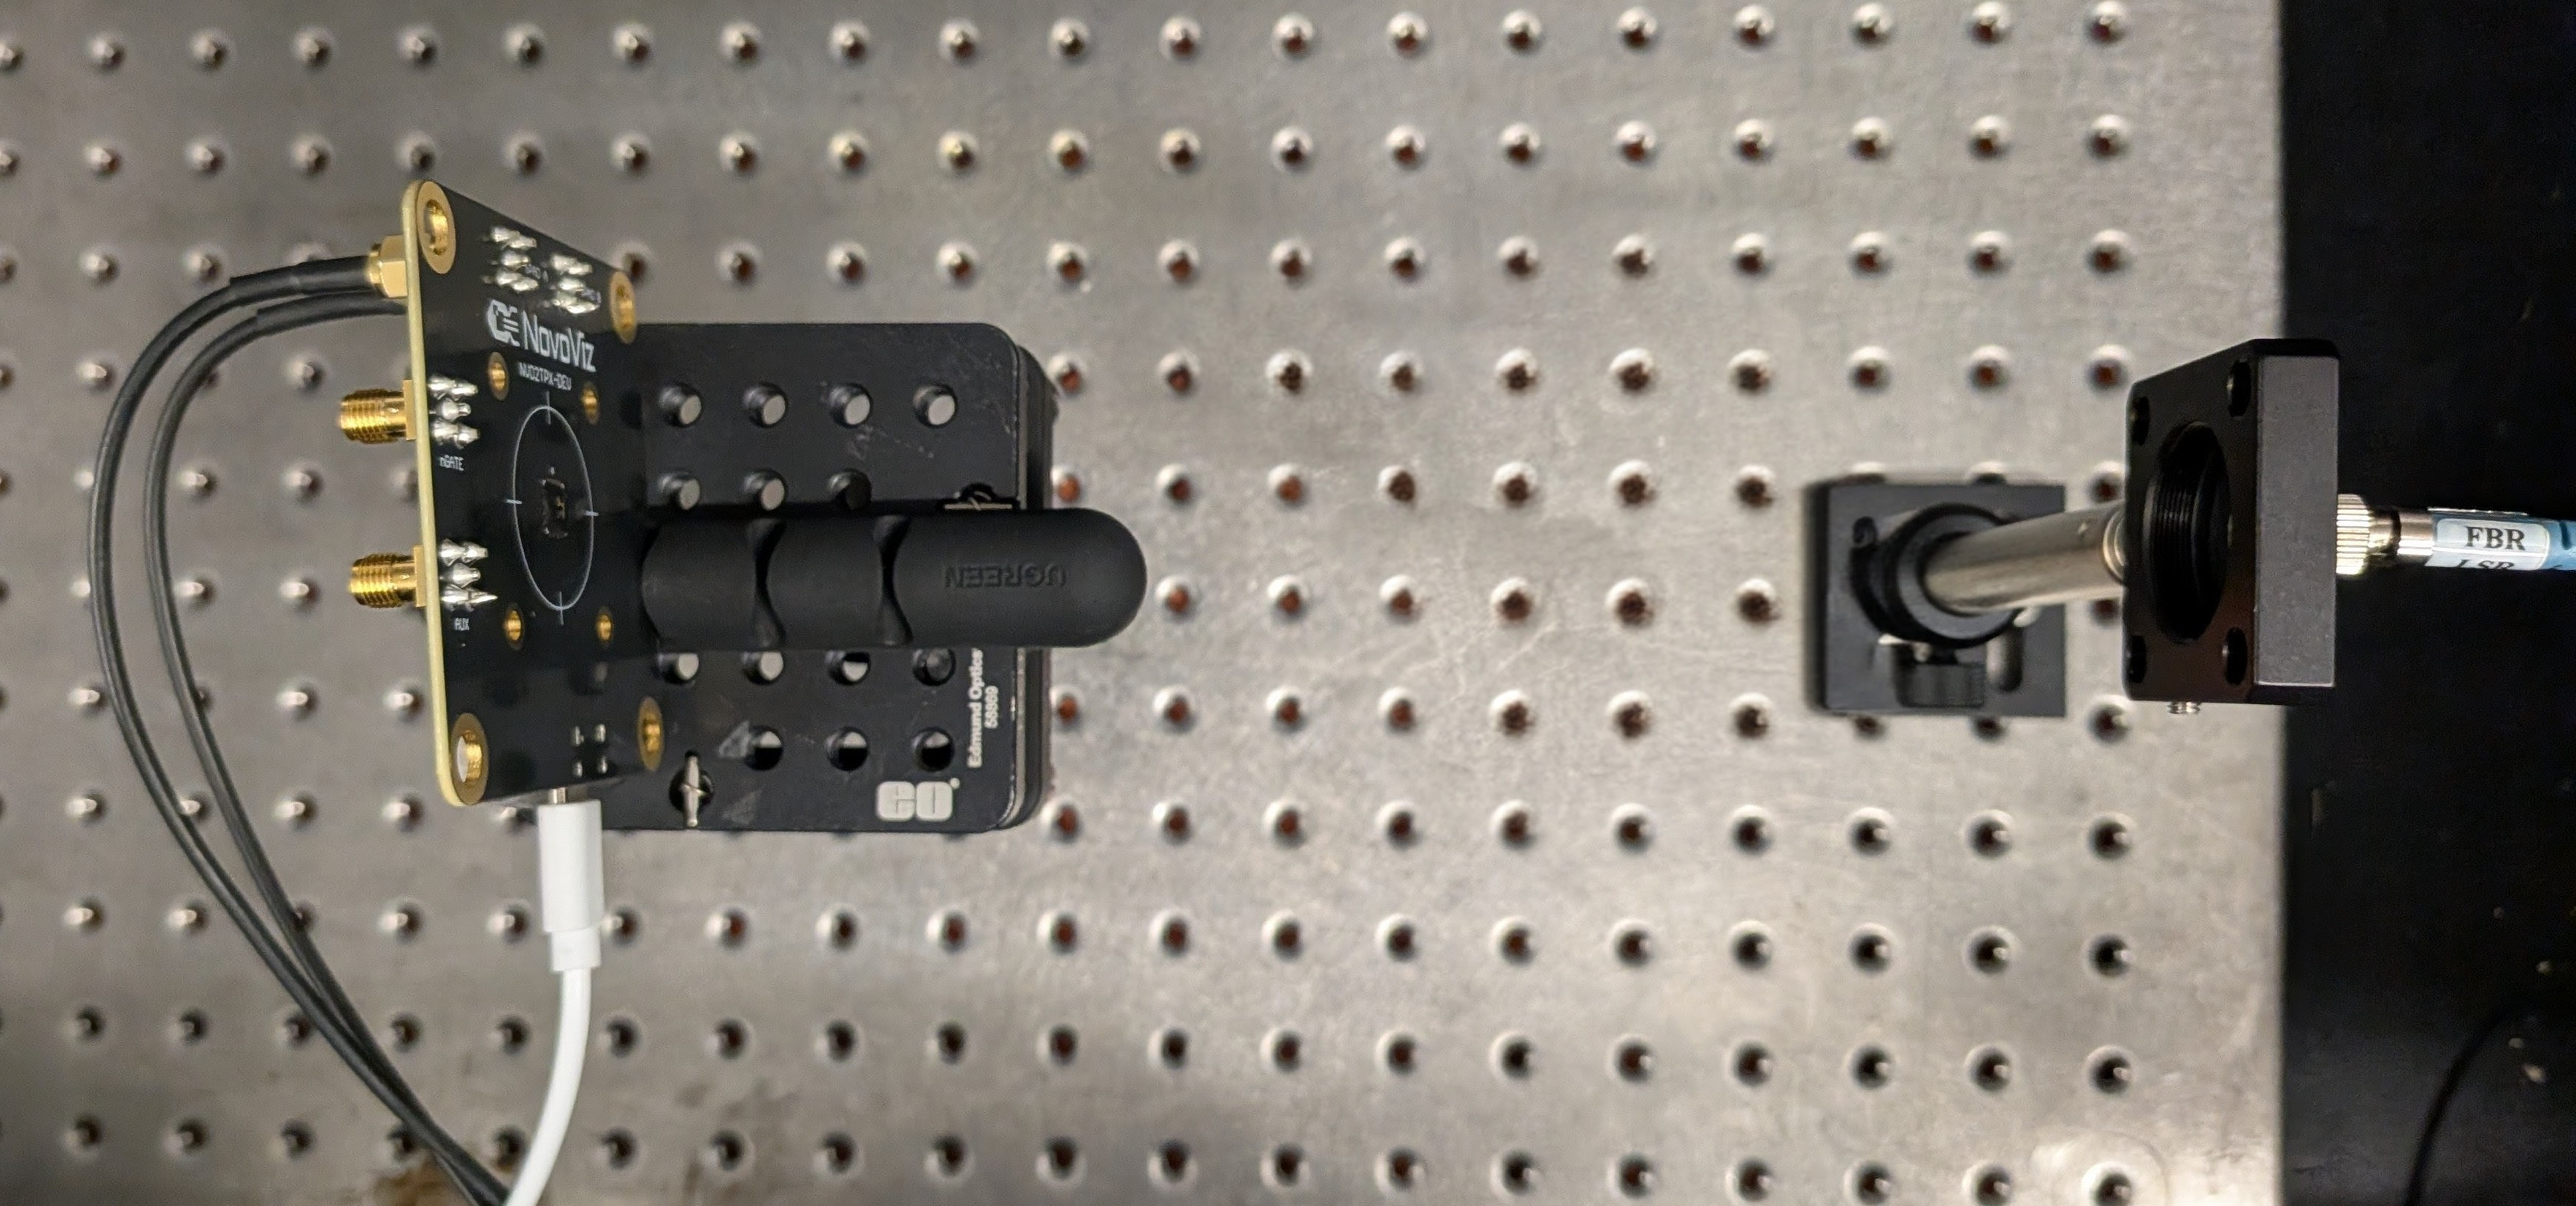
\includegraphics[width=0.45\textwidth]{Figures/exp_layout_plain.jpg}
    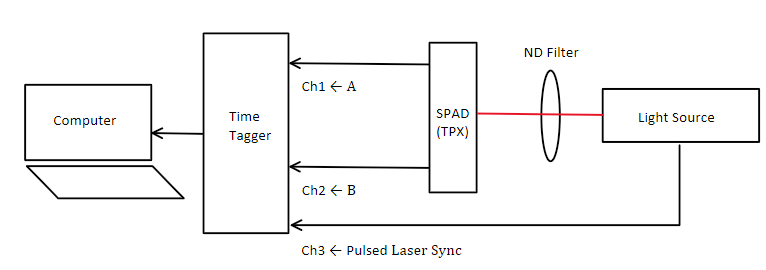
\includegraphics[width=0.45\textwidth]{Figures/exp_layout1_diagram.png}
    \caption{Experimental layout. Source is feed into the system with fiber optic cable that couples into free space with the \href{https://www.thorlabs.com/item/SM1FC2}{SM1 FC2} and irradiates the SPAD.}
    \label{fig:exp_lay}
\end{figure}

\subsection{TDC Application Programming Interface}
To process the timestamps generated by the single-photon detectors, this work utilizes the Swabian Instruments Time Tagger API \cite{swabian_correlation_web}, specifically the \href{https://www.swabianinstruments.com/static/documentation/TimeTagger/api/measurements/time_histograms.html#_CPPv411Correlation}{\texttt{tt.Correlation}} class. 
This function computes the cross-correlation between two detection channels. 

The algorithm operates within a user-defined correlation time window. 
This window is determined by specifying a temporal \texttt{bin width} and a total \texttt{number of bins}. 
For every photon event registered on a start channel, the algorithm calculates the time delay ($\tau$) to subsequent events on a stop channel, provided those events fall within the bounded correlation window. 
These computed delays are continuously accumulated and sorted into their respective time bins resulting in the final coincidence histogram, which is directly proportional to the second-order coherence function, $g^{(2)}(\tau)$.

\subsection{SPAD Characterization}
With the set up complete, a SPAD calibration is performed to verify the setup is operating within the expected margins. 
With an autocorrelation measurement we expect to extract a value for the dead time of the detector, and the afterpulsing probability and confirm that the digital pipeline is working as expected. 
The autocorrelation is measured with the \texttt{tt.Correlation} function with the same SPAD as the start and stop channel. 
The procedure is listed bellow: 
\begin{enumerate}
    \item Connect the CW laser source 1 to the fiber optics line feeding the system. 
    \item Connect the SPAD detectors with SMA Cables to Swabian Time Tagger. 
    \item Initialize the autocorrelation measurement (\texttt{tt.Correlation}) using a single SPAD channel as both the "start" and "stop" trigger. 
    \item Wait for detection events to accumulate for 10 seconds.
    \item Extract dead time and afterpulsing probabilities from data (See figure \ref{fig:autocorr}).
    \item Repeat 5 times to gather statistics. 
\end{enumerate}

\begin{figure}[htpb]
    \centering
    %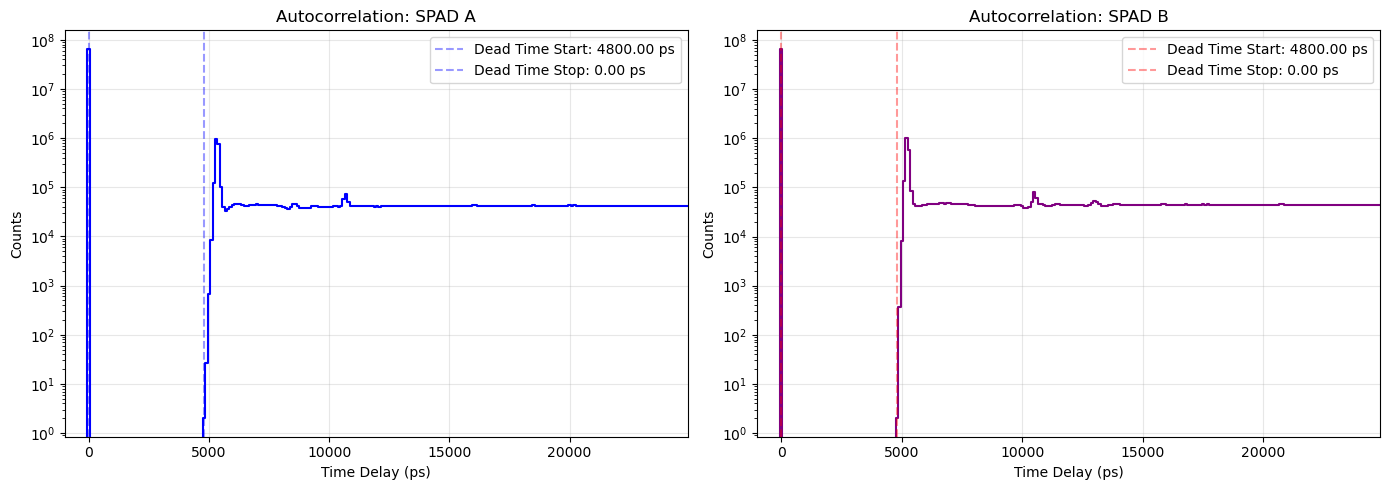
\includegraphics[width=0.5\textwidth]{Figures/autocorr_measurement.png}
    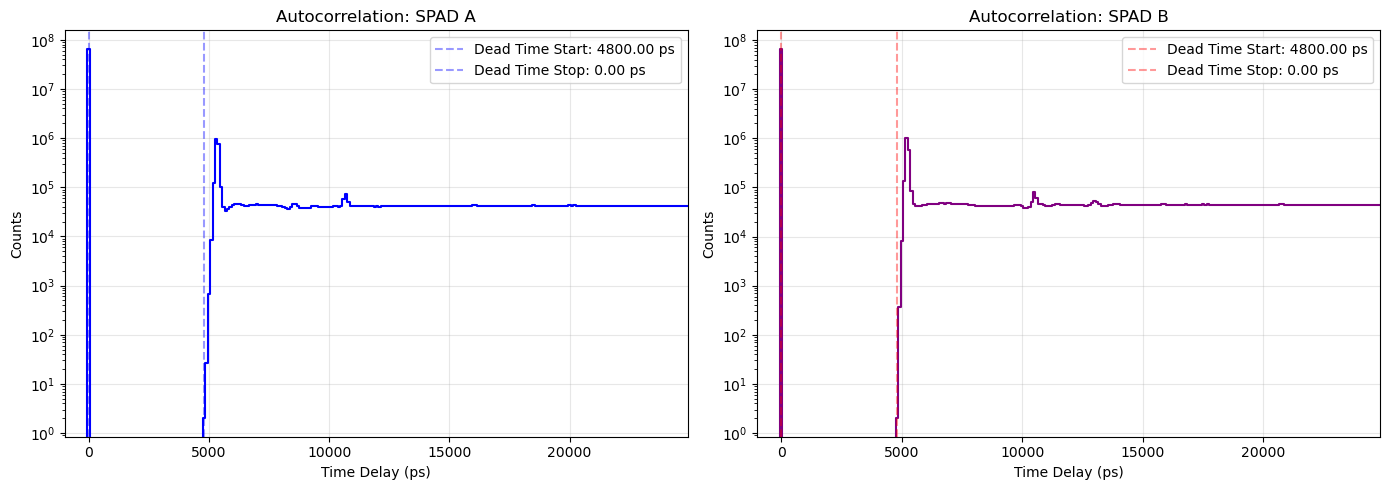
\includegraphics[trim=0cm 0cm 17.4cm 0cm, clip, width=\linewidth]{Figures/autocorr_measurement.png}
    \caption{Autocorrelation histogram of the SPAD channel 1. The measurement was taken with an illumination count rate of 10 Mcps and a histogram bin width of 100 ps.}
    \label{fig:autocorr}
\end{figure}

Figure \ref{fig:autocorr} shows the resulting autocorrelation histogram. 
The dead time is quantitatively defined as the temporal delay at which the coincidence counts recover from 0 counts. 
To calculate the afterpulsing probability ($P_{ap}$), the steady-state baseline counts are first estimated from the flat region of the histogram occurring well after the detector recovery. 
This baseline is subtracted from the total counts to isolate the excess detections. $P_{ap}$ is then determined by integrating these excess counts from the end of the dead time ($t_{dt}$) to the end of the time window ($t_{end}$), normalized by the total number of valid trigger events ($N_{triggers}$):

\begin{equation}
    P_{ap} = \frac{\sum_{t = t_{dt}}^{t_{end}} (N_{counts}(t) - N_{baseline})}{N_{triggers}}
\end{equation}

The results of this characterization are summarized in Table \ref{tab:calibration_summary}.

\begin{table}[htpb]
    \centering
    \caption{Summary of Detector Calibration Parameters}
    \label{tab:calibration_summary}
    \resizebox{\linewidth}{!}{%
    \begin{tabular}{lcc}
        \toprule
        \textbf{Parameter} & \textbf{SPAD 1} & \textbf{SPAD 2} \\
        \midrule
        %DCR (cps) & $9.74 cps$ & $10,301.49$ \\
        Mean Dead Time (ns) & $4.90 \pm 0.12$ & $4.85 \pm 0.09$ \\
        Maximum Repetiton Rate (MHz) & 204.08 & 206.19 \\
        Afterpulsing Probability (\%) & 2.41 & 2.30 \\
        \bottomrule
    \end{tabular}
    }
\end{table}
